\chapter{Simulation}
Die Simulationen sind vom Grundaufbau her wie folgt implementiert: Sie bestehen aus einem Konfigurationsskript, das die Parameter für das eigentliche Modell in den Matlab Workspace lädt und die Automatisierung der Simulationsläufe implementiert. Das Modell wird in Simulink über das PLECS Blockset aufgebaut und die Daten werden über eine Ausgabe als gebündelte Schnittstelle an Matlab zurückgegeben. Die Rückführung der Daten erfolgt einheitlich für die Simulationen in einer festgelegten Reihenfolge, siehe Abb. \ref{fig:plecsout}. Dies ermöglicht eine einheitliche Auswertung und Speicherung der Daten, zur Begrenzung der Datenmenge wird die Anzahl der Messpunkte auf die letzte Sinusperiode begrenzt. Die Schaltung und die zugehörige Steuerung befinden sich in jeweils eigenen PLECS-Systemen, für das Netz und den Elektrolyseur ist ein eigenes Subsystem vorgesehen, siehe Abbildung \ref{fig:plecssimulationsaufbau}.  
\begin{figure}[H]
\centering
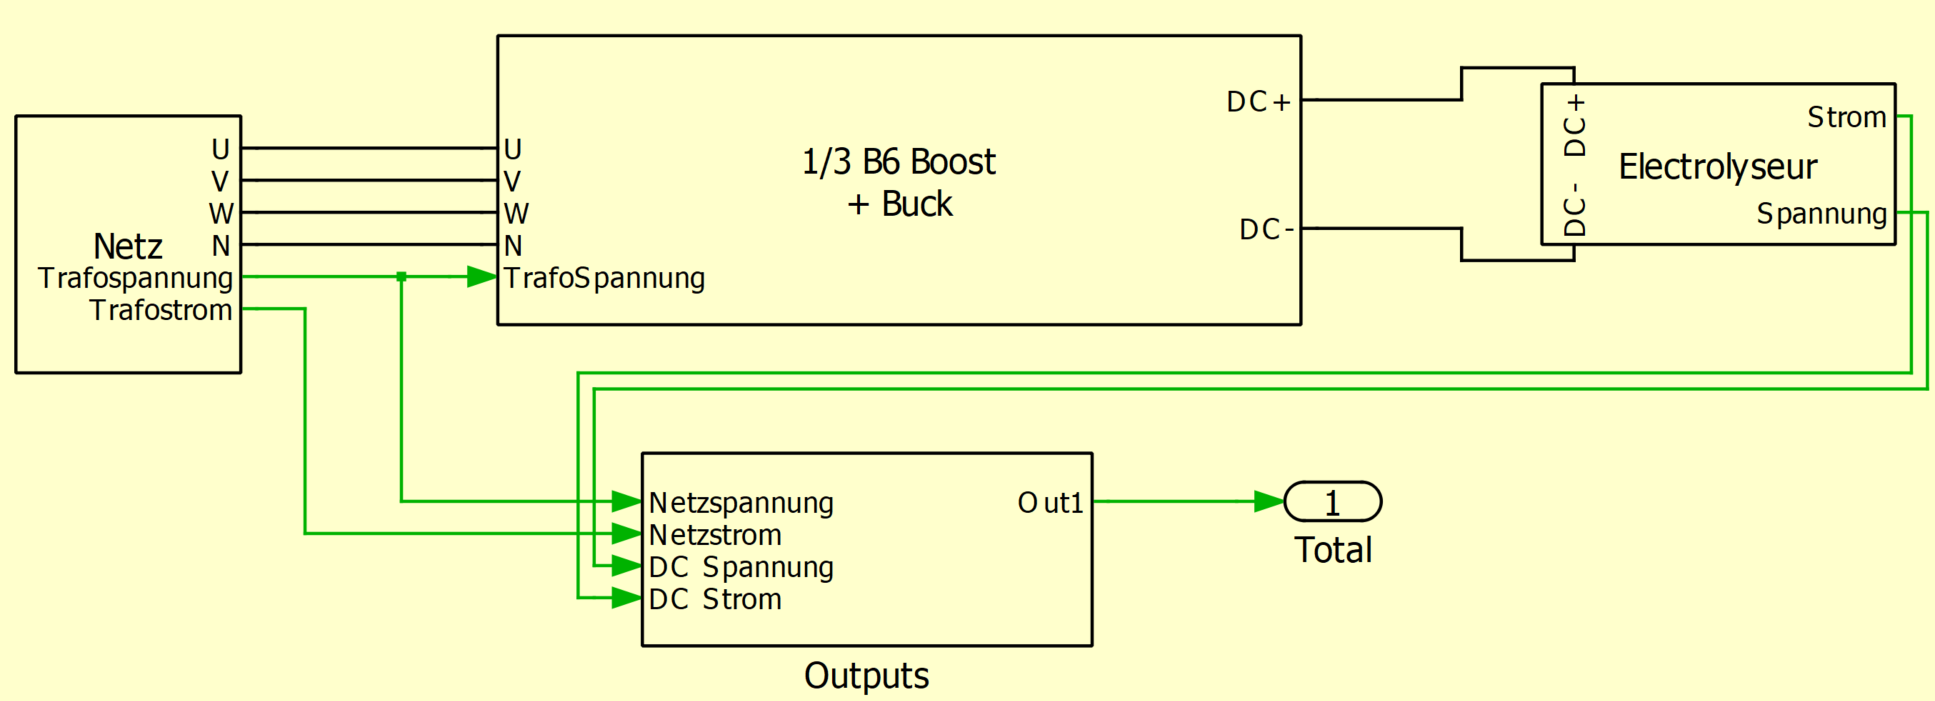
\includegraphics[width=1\linewidth]{content/Grafiken/PLECS_Simulationsaufbau}
\caption{Übersicht der PLECS Simulation}
\label{fig:plecssimulationsaufbau}
\end{figure}
Das Netz wird durch eine einfache Drehstromquelle dargestellt und kann in späteren Schritten durch Netzimpedanzen und Fehlerszenarien ergänzt werden. Der Elektrolyseur besteht der Einfachheit halber aus einem geeigneten Lastwiderstand, der im Betriebspunkt die gemäß Skript eingestellte Leistung aufnimmt. Zusätzlich werden einige Widerstände verwendet, um die Schaltung in \gls{PLECS} berechenbar zu machen, da sonst beim Einschaltvorgang durch Kapazitäten unendlich hohe Ströme entstehen würden und in der realen Anlage immer parasitäre Widerstände vorhanden sind.
\begin{figure}
\centering
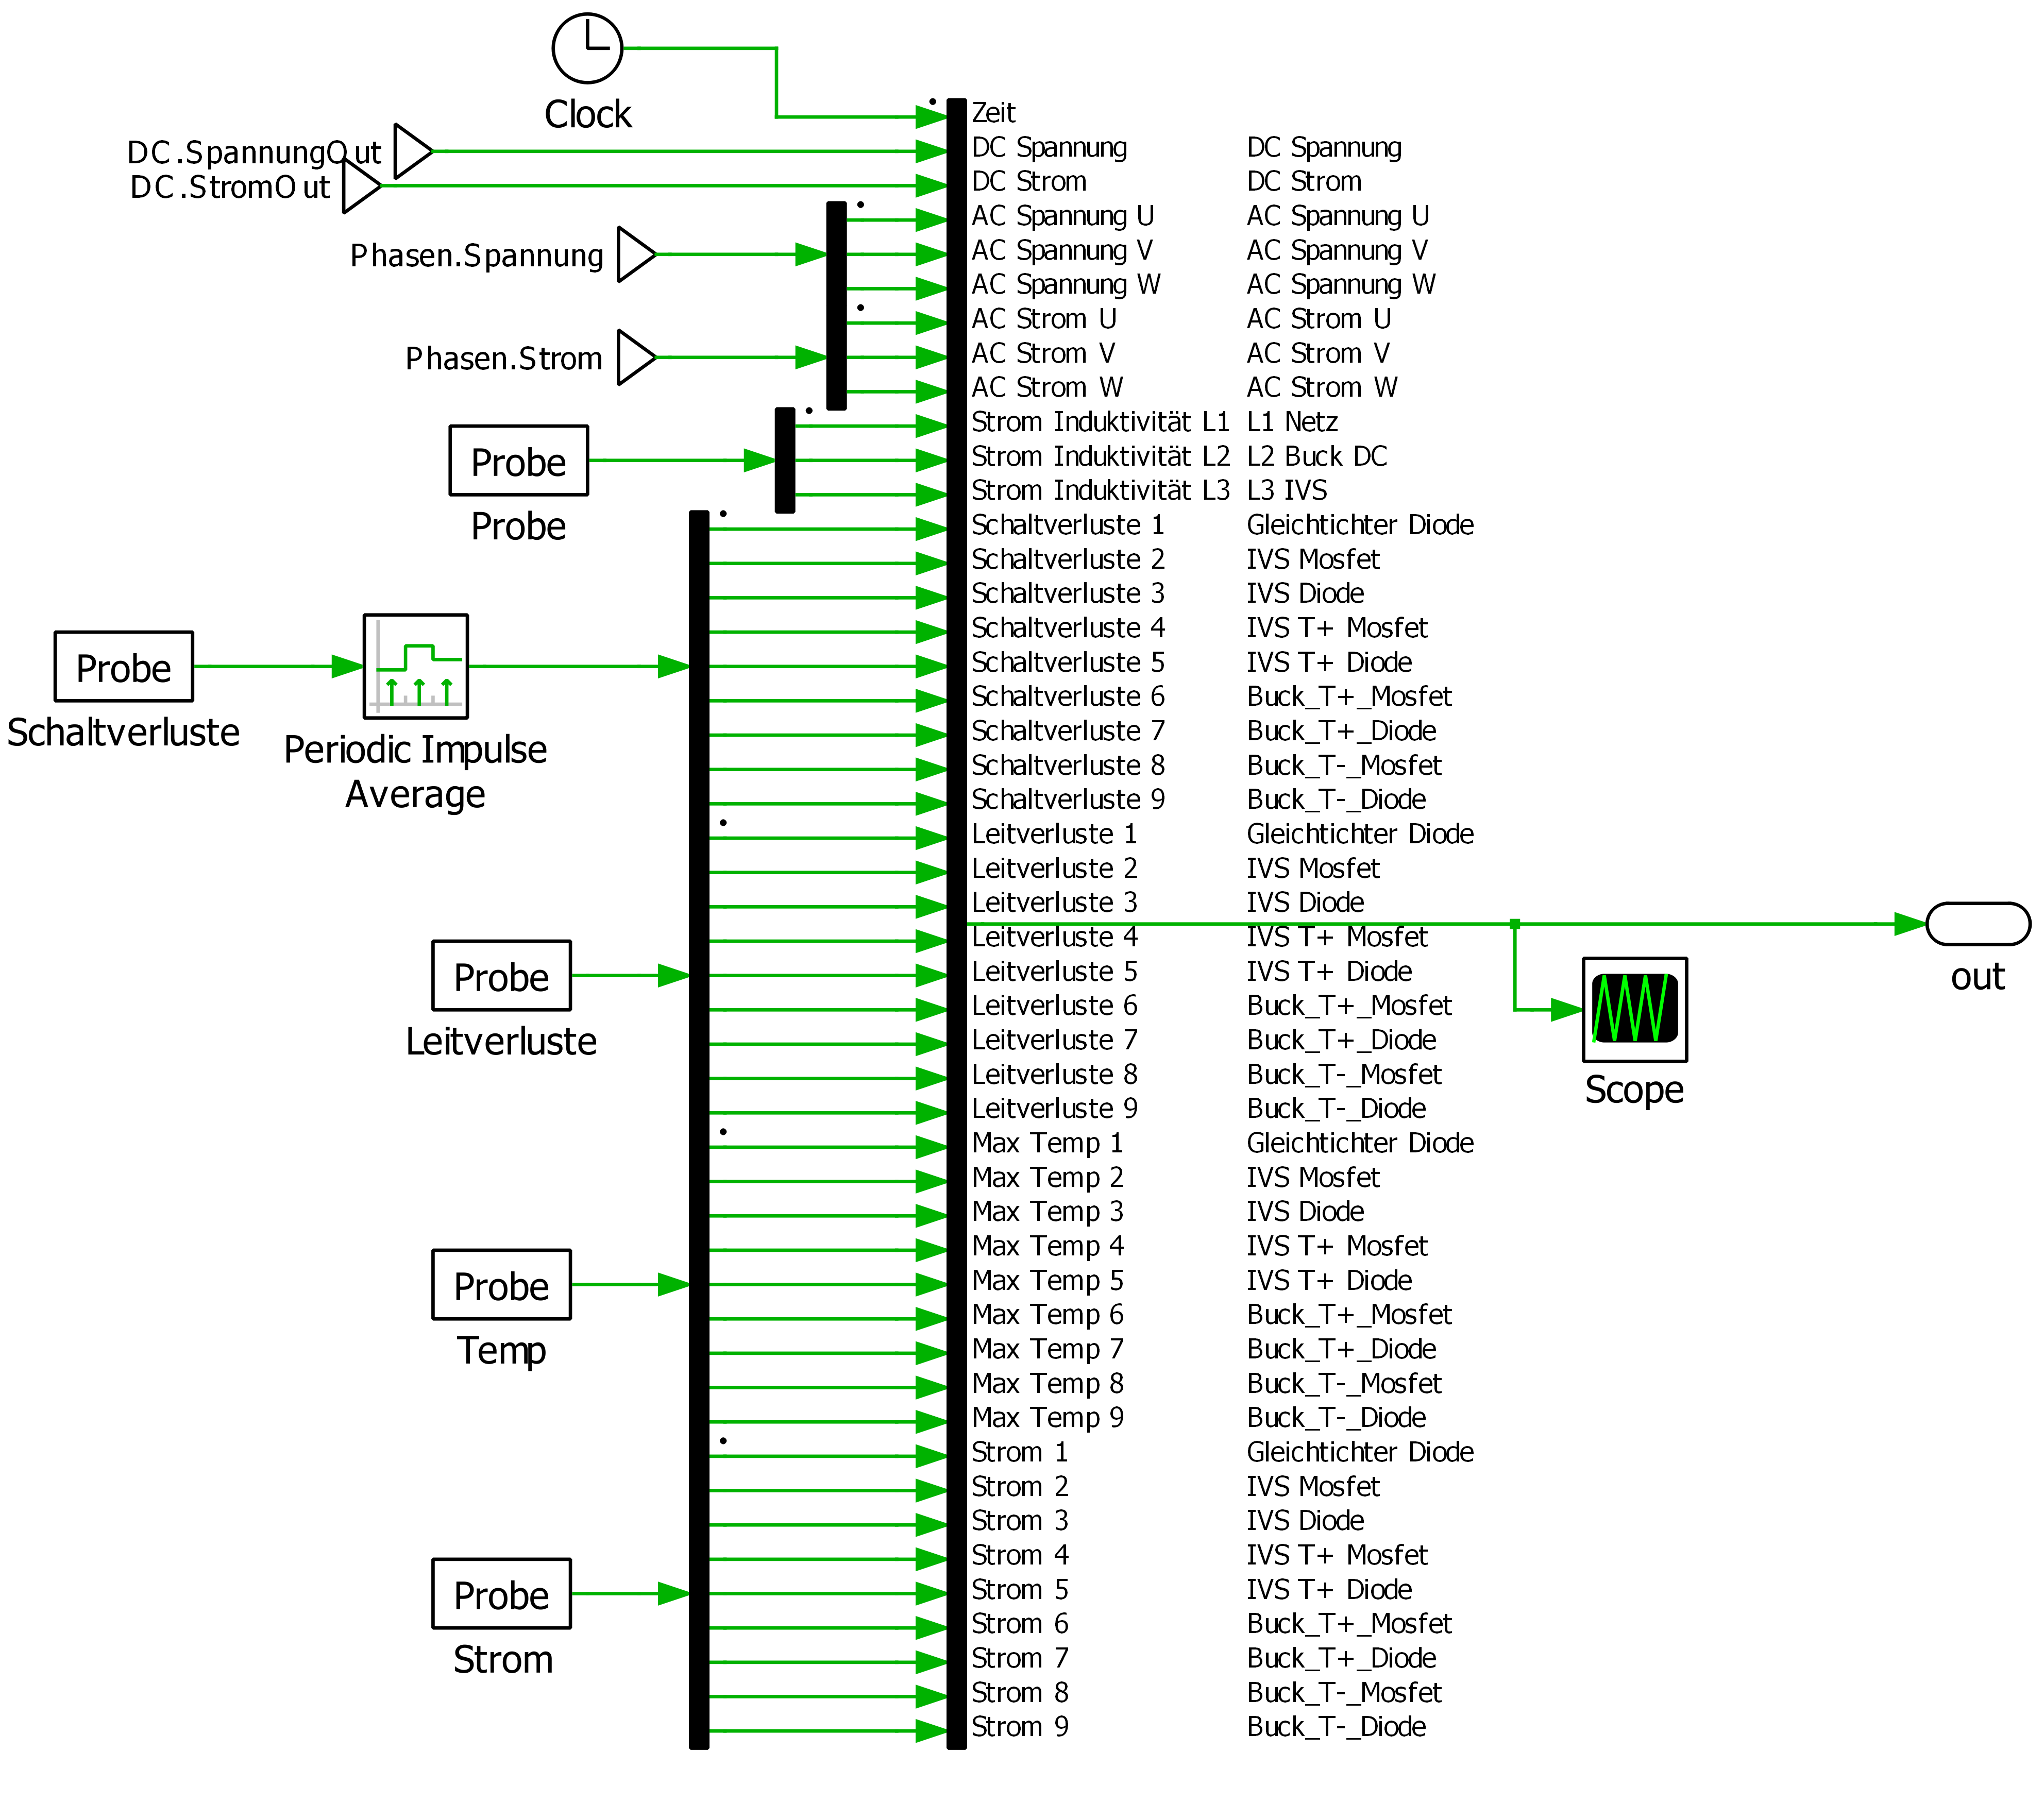
\includegraphics[width=1\linewidth]{content/Grafiken/Plecs_Out}
\caption{Zusammenfassung der Simulationsoutputs}
\label{fig:plecsout}
\end{figure}


\section{Randbedingungen}
Für den Gleichrichter werden grundlegende Parameter festgelegt, um die Auslegung für die Simulation durchführen zu können. Die Leistung von 200 kW wird als Grundlage festgelegt, da aufgrund der Halbleiter Module und thermischen Belastung höhere Ströme in einem Gerät Probleme bei der Umsetzung bereiten würden. Halbeitermodule die aktuell industriell für Platinen-basierte Stromrichter eingesetzt werden, können Ströme von maximal 200 A führen. Die Ausgangsspannung von maximal 680 V ergibt sich aufgrund der Spannungsfestigkeit der Halbleitermodule, welche 1200 V beträgt, durch Schalt-transienten treten höhere Spannungen an den Halbleitern auf als die eigentliche Ausgangsspannung. Aufgrund von Unsicherheiten im Schaltvorgang kann es zu Überspannungen kommen, welche die Halbleiter Lebensdauer beeinträchtigen kann, weshalb ein größerer Abstand zur Halbleiterspannung gewählt wird. Es wird sich für diese Spannungsklasse entschieden, da diese bereits etabliert und in breiter Masse verfügbar ist. Die Netzfrequenz sowie Spannungsschwankung wird anhand der Anforderungen für Stationären Betrieb im deutschen Stromnetz definiert. Die Spannungsschwankung wird auf 10 \% reduziert da kurzfristige Änderungen und entsprechende Kompensationen später betrachtet werden.  \\

\begin{itemize}
\item \gls{Pa}: 200 kW
\item \gls{Ua}: 482-680 V
\item \gls{Ia}: 	295 A
\item \gls{Ull}:		617 V
\item Netzfrequenz		50 Hz
\item Filterblindleistung: 3 \%
\item \gls{fs}: 20 kHz
\item Netzspannungsschwankung: 10 \%
\end{itemize}

Für die Auswertung wird der eingeschwungene Zustand des Systems betrachtet. Dies erleichtert die Auslegung der Regler, die Parameter werden so gewählt, dass ein stabiler Zustand erreicht wird und keine Schwingungen oder ähnliches auftreten. Außerdem wird für die Auswertung die letzte Periode der Simulation verwendet, dieser Abschnitt wird für eine spätere Betrachtung gespeichert.

\section{Tiefsetzsteller}
Der Tiefsetzsteller kann in den beiden Kreisen entkoppelt betrachtet werden, was für die Auslegung der Induktivität von Vorteil ist. Die Regelung kann ebenfalls entkoppelt erfolgen, so dass eine getrennte Stabilitätsbetrachtung und Optimierung möglich ist. 
	\subsection{Auslegung der Induktivität}
	Die Speicherdrossel wird nach der Formel \ref{eq:BuckL} ausgelegt, wobei die Netzspannung maximal $U_{LLmaxPeak}=1,1 \cdot 617 \si{\V} \cdot \sqrt{2}=959,8 \si{\V}$ und die Ausgangsspannung $U_{amin}$ bei mindestens 482 \si{\V}. Daraus ergeben sich die maximalen Parameter, die der Tiefsetzsteller realisieren muss. Es ergibt sich eine Induktivität von 134,16 \si{\micro \henry}, siehe Formel \ref{eq:BuckLwert}. Die Energie beträgt 7,78 Joule bei einem Ausgangsstrom von 294 A. 
	\begin{equation}
	\label{eq:BuckLwert}
	L_{T}= \dfrac{U_{LLmaxPeak}-U_{amin}}{f_{sw} \cdot \Delta I} \cdot D = \dfrac{959,8\si{\V} - 482 \si{\V}}{20 \si{\kilo \hertz}\cdot 0,3 \cdot 295 \si{\ampere}} \cdot \dfrac{482 \si{\V}}{959,8 \si{\V}}= 134,16 \si{\micro \henry} 
	\end{equation}
	\begin{equation}
		E=1/2 \cdot L_{T} \cdot I_{a}^{2} = 1/2 \cdot 134,16 \si{\micro \henry}  \cdot 294 \si{\ampere} = 7,78 J
	\end{equation}
	\subsection{Regelung}
	Die Regelung kann mit den im Abschnitt \ref{sec:Buck} beschriebenen Eingangsspannungsverhältnissen ausgelegt werden, der Duty Cycle \gls{D} ist das Verhältnis von Eingangsspannung zu Ausgangsspannung. Aufgrund der sechspulsigen Zwischenkreisspannung schwankt der Duty Cycle \gls{D} geringfügig, da aber eine feste Ausgangsspannung gewünscht ist, kann die Regelung mit einem PI-Regler realisiert werden.\\
	Der Tiefsetzsteller wird durch einen PI-Regler zur Fehlerkorrektur angesteuert, wobei der ideale Tastgrad aus der gewünschten Ausgangsspannung und der Zwischenkreisspannung \gls{Upn} bestimmt wird. Die gewünschte Ausgangsspannung \gls{Ua} wird durch den Sollstrom und den bekannten Lastwiderstand generiert. Das Tastverhältnis wird dann einem PWM-Generator zugeführt, der das Signal mit der gewünschten Schaltfrequenz von 20 kHz erzeugt. Um die Schaltverluste und insbesondere die Leitungsverluste beim Kommutieren in den Dioden zu berücksichtigen, wird eine Totzeit von 500 \si{\nano \second} eingestellt, siehe Abbildung. \ref{fig:iafbuckcontrol}.
	\begin{figure}[H]
		\centering
		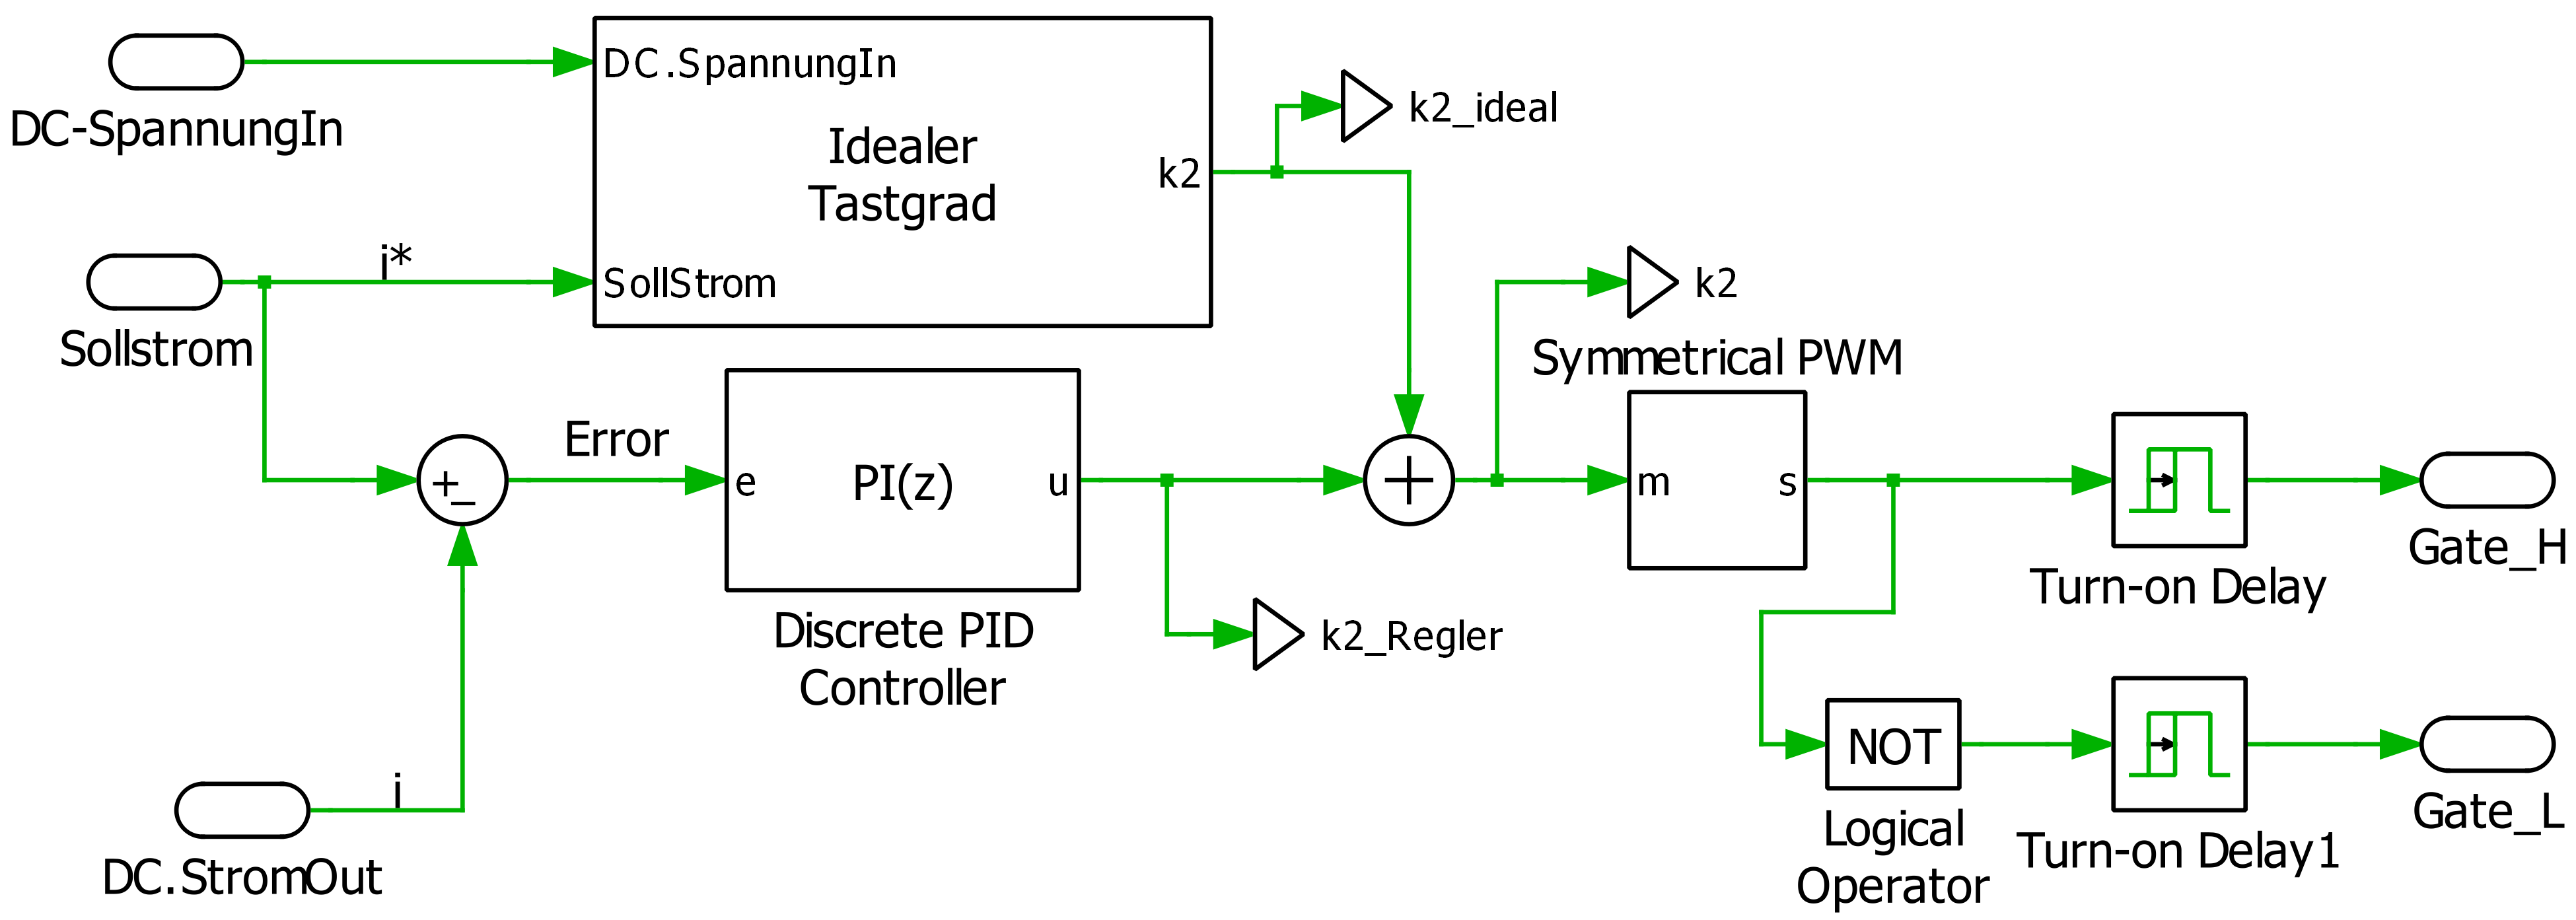
\includegraphics[width=1\linewidth]{content/Grafiken/IAF_BuckControl}
		\caption{Regelung des Tiefsetzstellers des IAF}
		\label{fig:iafbuckcontrol}
	\end{figure}


\section{IAF}
	Der Schwerpunkt der Simulation liegt auf den Leistungshalbleitern, deren Anordnung in Abbildung \ref{fig:iafplecsmain} und \ref{fig:iafplecsivs} zu entnehmen ist. Zur Bestimmung der Verlustleistung werden Modelle von Infineon verwendet, wobei für die Dioden und den \gls{IVS} ein gemeinsames Modul mit 5 \si{\milli \ohm} \gls{SiC} \gls{MOSFET}. Die Halbbrücke an der Induktivität wird aus einem Modul mit 13 \si{\milli \ohm} aufgebaut. Alle Halbleiter haben eine Spannungsfestigkeit von 1200 V.
	\begin{figure}
		\centering
		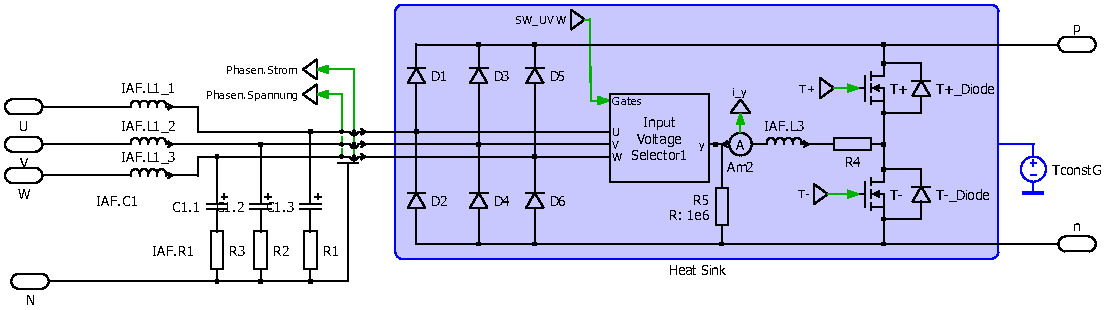
\includegraphics[width=1\linewidth]{content/Grafiken/IAF_Plecs_main}
		\caption{Simulationsaufbau der Halbleiter des IAF}
		\label{fig:iafplecsmain}
	\end{figure}
	\begin{figure}
		\centering
		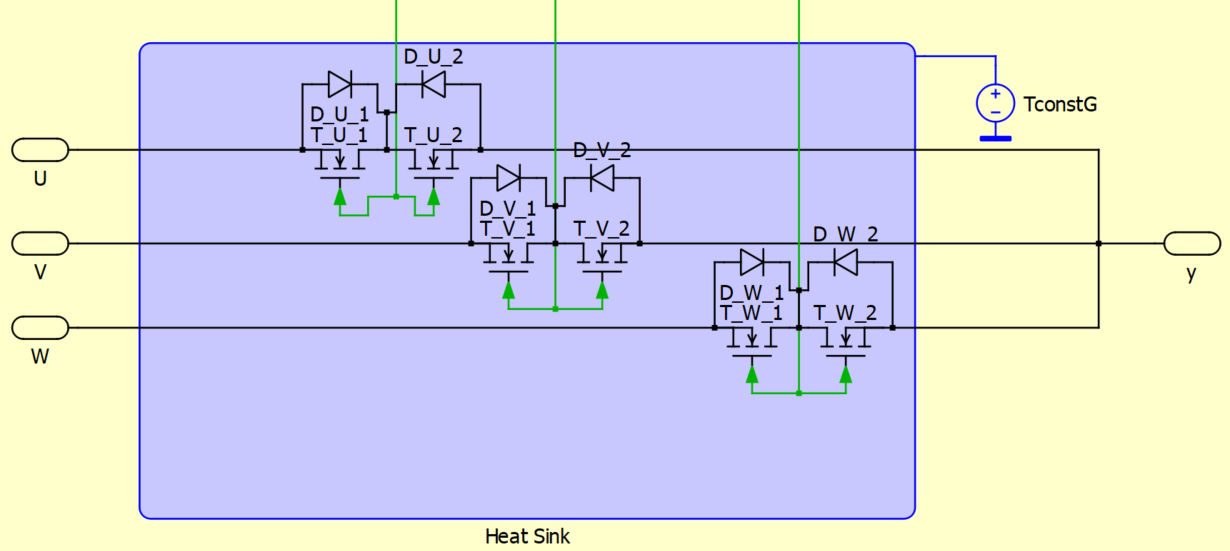
\includegraphics[width=1\linewidth]{content/Grafiken/IAF_Plecs_IVS}
		\caption{Simulationsaufbau der Halbleiter des IVS vom IAF}
		\label{fig:iafplecsivs}
	\end{figure}
	

	\subsection{Auslegung der Induktivitäten}
	Der maximale Rippelstrom ergibt sich aus der maximalen Leistung und der minimalen Netzspannung und beträgt 44,1 \si{\A}, siehe Formel \ref{eq:DeltaIIVS}. Der Rippelstrom ist wiederum auf 30 \% des Nennstroms ausgelegt. Daher muss die Induktivität einen Wert von 272 \si{\micro \henry} haben, siehe Formel \ref{eq:Livs}. 
		
		\begin{equation}
		\label{eq:DeltaIIVS}
		I_{\Delta max IVS}=\dfrac{0,3\cdot \sqrt{2} \cdot P_{a}}{2 \cdot \sqrt{3} \cdot U_{LL} \cdot 0,9} = \dfrac{0,3\cdot \sqrt{2} \cdot 200 \si{\kilo \watt}}{2 \cdot \sqrt{3} \cdot 617 \si{V} \cdot 0,9} = 44,1 \si{\A}
		\end{equation}
		
		\begin{equation}
			\label{eq:Livs}
			L_{IVS}= \dfrac{U_{LLmaxPeak}}{4\cdot f_{sw} \cdot I_{\Delta max IVS}} = \dfrac{959,8 V}{4 \cdot 20 kHz \cdot 44,1 A}= 272 \si{\micro \henry}
		\end{equation}
		
		Bei der Betrachtung der Energie ist zu beachten, dass der Strom in der Drossel bei Blindleistung ansteigt und somit die Energie im quadratischen Verhältnis zunimmt. Der Strom bei einer Phasenverschiebung von 30 Grad wird über den Faktor $sin(30)=0,5$ berechnet und ergibt sich somit zu 132,33 A (siehe Formel \ref{eq:IAF_I30}).
		\begin{equation}
			\label{eq:IAF_I30}
			I_{IAF30°}=\dfrac{0,5\cdot \sqrt{2} \cdot 200 \si{\kilo \watt}} { \sqrt{3} \cdot 617 \si{V}} = 132,33 \si{\A}
		\end{equation}
		Die in der Drossel gespeicherte Energie, welche eine relevante Größe für die Bewertung darstellt, beträgt 2,38 Joule (siehe Formel \ref{eq:EL_IVS}).
		\begin{equation}
			\label{eq:EL_IVS}
			E_{IVS}=0,5 \cdot L_{IVS} \cdot I_{\Delta max IVS}^{2} = 0,5 \cdot 272 \si{\micro \henry} \cdot (44,1 \si{\A})^{2} =  2,38 J
		\end{equation}
		
		
		Zusätzlich wird eingangsseitig eine Filterinduktivität mit dem Wert 1 \si{\micro \henry} eingesetzt, diese hat eine gespeicherte Energie von 0,1 Joule, siehe Formel \ref{eq:E_IAF_ACL}. Aufgrund der dreiphasigen Anwendung wird der Wert direkt mit dem Faktor 3 multipliziert.
			\begin{equation}
			\label{eq:E_IAF_ACL}
			E_{L-IAF-AC}=3\cdot 0,5 \cdot 1 \si{\micro \henry} \cdot (260 \si{\ampere})^{2} = 0,1 J
		\end{equation}
	
	\subsection{Regelung}
		
		
		Die Regelung des Stroms des IVS wird anhand der Struktur von Soeiro et al. umgesetzt (vgl. Abb. ef{fig:iafpapercontrol}) \cite{Soeiro.2013}. 
		 \begin{figure}[H]
			\centering
			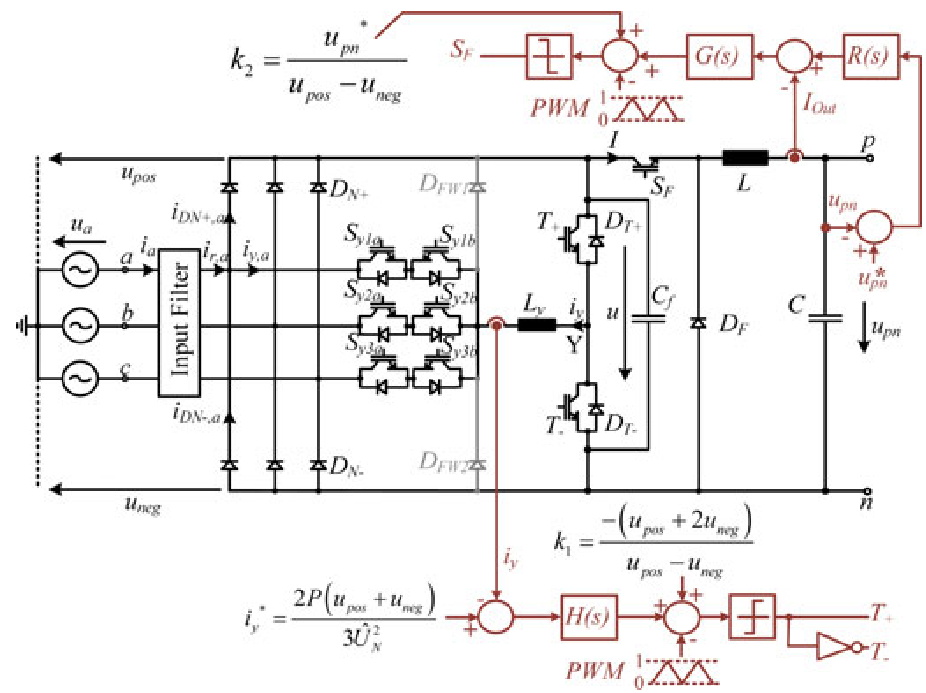
\includegraphics[width=0.8\linewidth]{content/Grafiken/IAF_Paper_Control}
			\caption{Struktur der Regelung des IAF \cite{Soeiro.2013}}
			\label{fig:iafpapercontrol}
		\end{figure}
		Die Umschaltung zwischen den Phasen erfolgt mithilfe einer vorhandenen PLL in PLECS zur Winkelbestimmung und anschließenden Sektorbestimmung. Die Sektorenzuweisung wird anhand des Phasenwinkels nach dem Schema aus Abbildung \ref{fig:b6iafsectors} umgesetzt. Die Auswahl der entsprechenden Schalter wird über ein C-Skript implementiert (siehe Abbildung \ref{fig:plecsiafivscontrol}). 
		\begin{figure}[H]
			\centering
			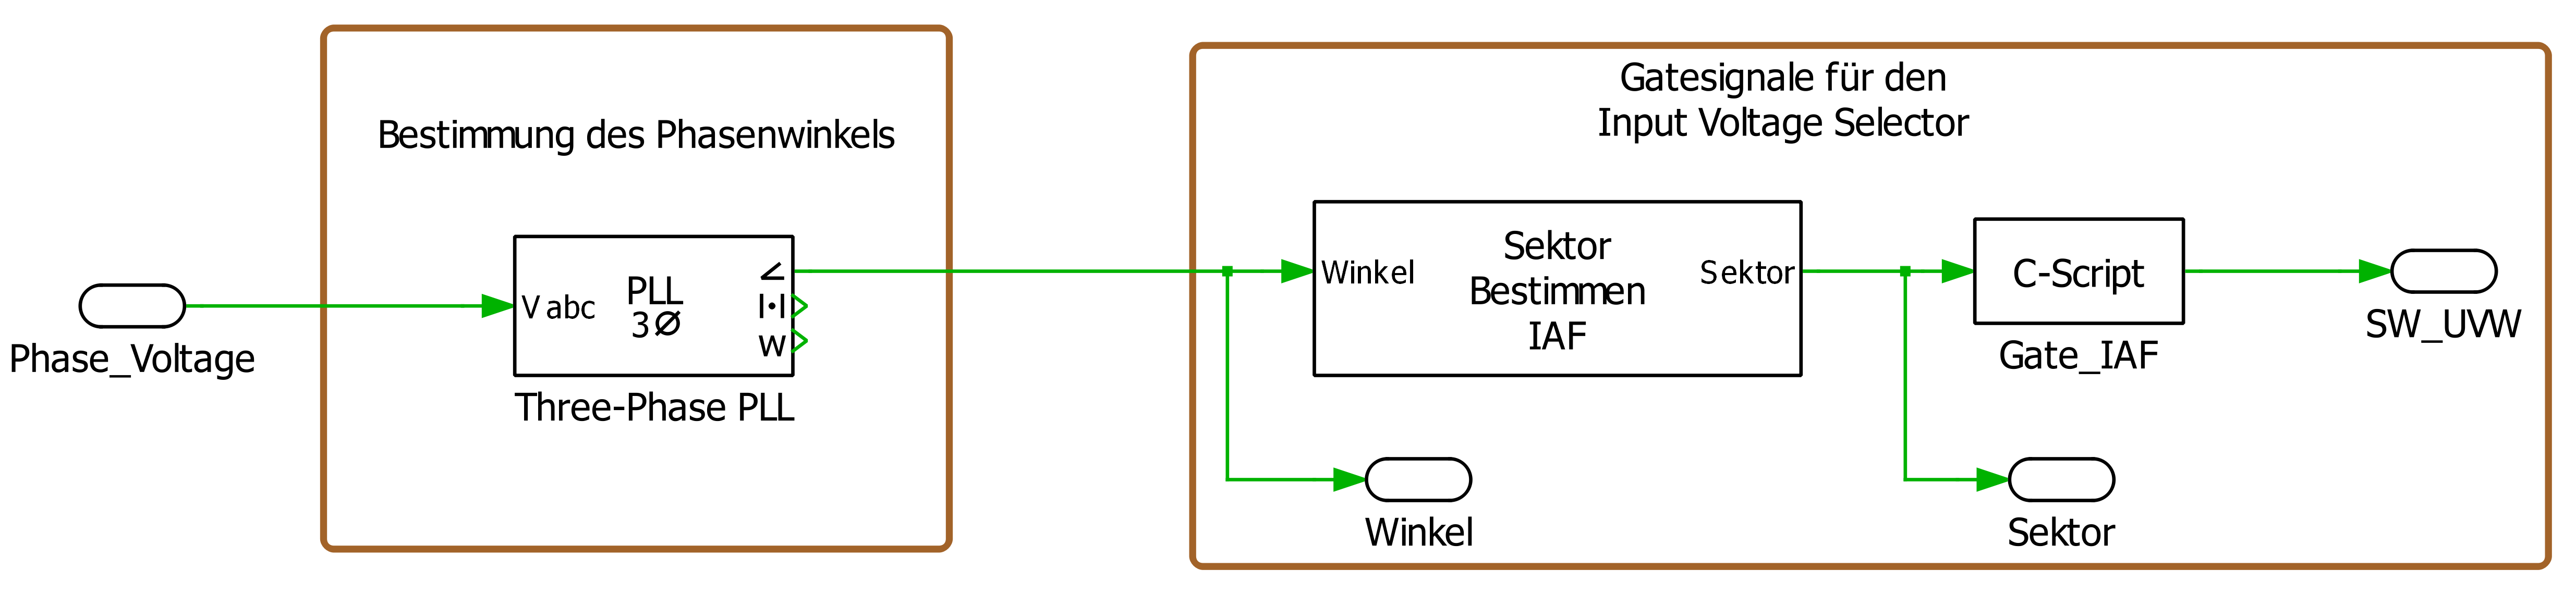
\includegraphics[width=1\linewidth]{content/Grafiken/PlecsIAFivscontrol}
			\caption{PLECS Aufbau der \gls{IVS} Ansteuerung}
			\label{fig:plecsiafivscontrol}
		\end{figure}
		Der optimale Tastgrad K1 für den Strom in der Drossel wird über das Verhältnis der Spannungen durch den formelmäßigen Zusammenhang in Gleichung \ref{eq:K1} bestimmt. 
		

		
		\begin{equation}
			\label{eq:K1}
			K1 = \dfrac{U_{mid}- U_{low}}{U_{high} -U_{low}} 
		\end{equation}
		
			Der Strom in der Drossel wird durch den aktuellen Phasenwinkel der Spannung erzeugt, welcher in der Ansteuerung des IVS durch die PLL erfasst wird und mit einer einstellbaren Phasenverschiebung verändert werden kann. Die Stromamplitude wird dabei über die Netzspannung und die gewünschte Ausgangsleistung bestimmt (siehe Formel \ref{eq:Idach}). Der sinusförmige Strom wird durch die Amplitude und den entsprechenden Winkel erzeugt. Die mittlere Phase wird über die Sektorenzuweisung ausgewählt. Siehe Abbildung \ref{fig:plecsiafiy}. 
		
		\begin{equation}
			\label{eq:Idach}
			 \hat{I} = \dfrac{\sqrt{2} \cdot P   }{ \sqrt{3} \cdot cos(\varphi) \cdot  U_{LLrms} }
		\end{equation}
		
		\begin{figure}
			\centering
			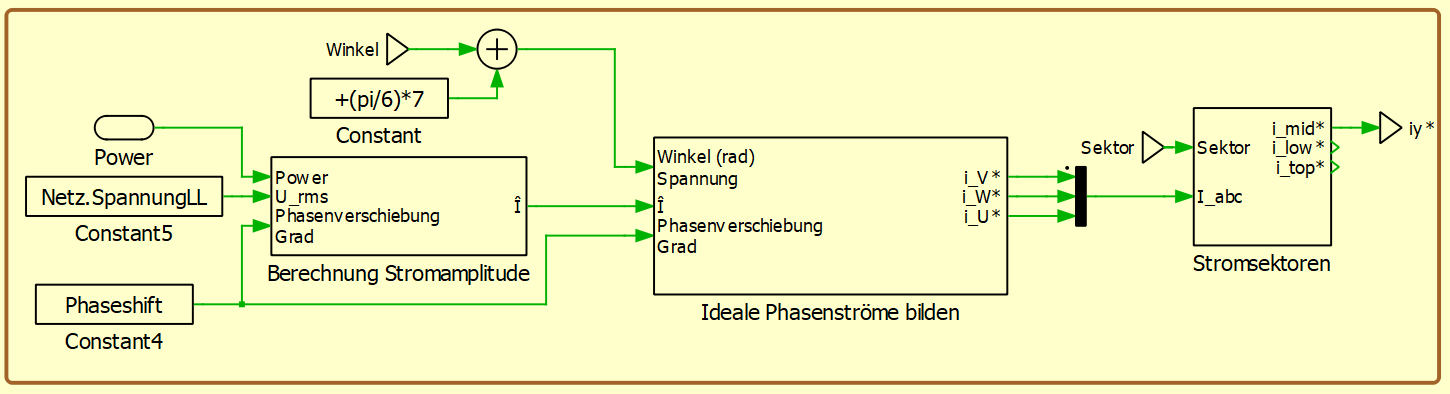
\includegraphics[width=1\linewidth]{content/Grafiken/PlecsIAFiy}
			\caption{Bestimmung des Sollstroms der mittleren Phase}
			\label{fig:plecsiafiy}
		\end{figure}
		
Die Stromregelung erfolgt mithilfe eines diskreten PI-Reglerblocks aus der PLECS-Bibliothek. Die Signale zur Gate-Ansteuerung werden durch einen PWM-Generator erzeugt und anschließend durch eine Einschaltverzögerung zur Totzeit-Implementierung verzögert. Dieser Aufbau ist in Abbildung \ref{fig:plecsiafivsk1} dargestellt. 
		\begin{figure}
			\centering
			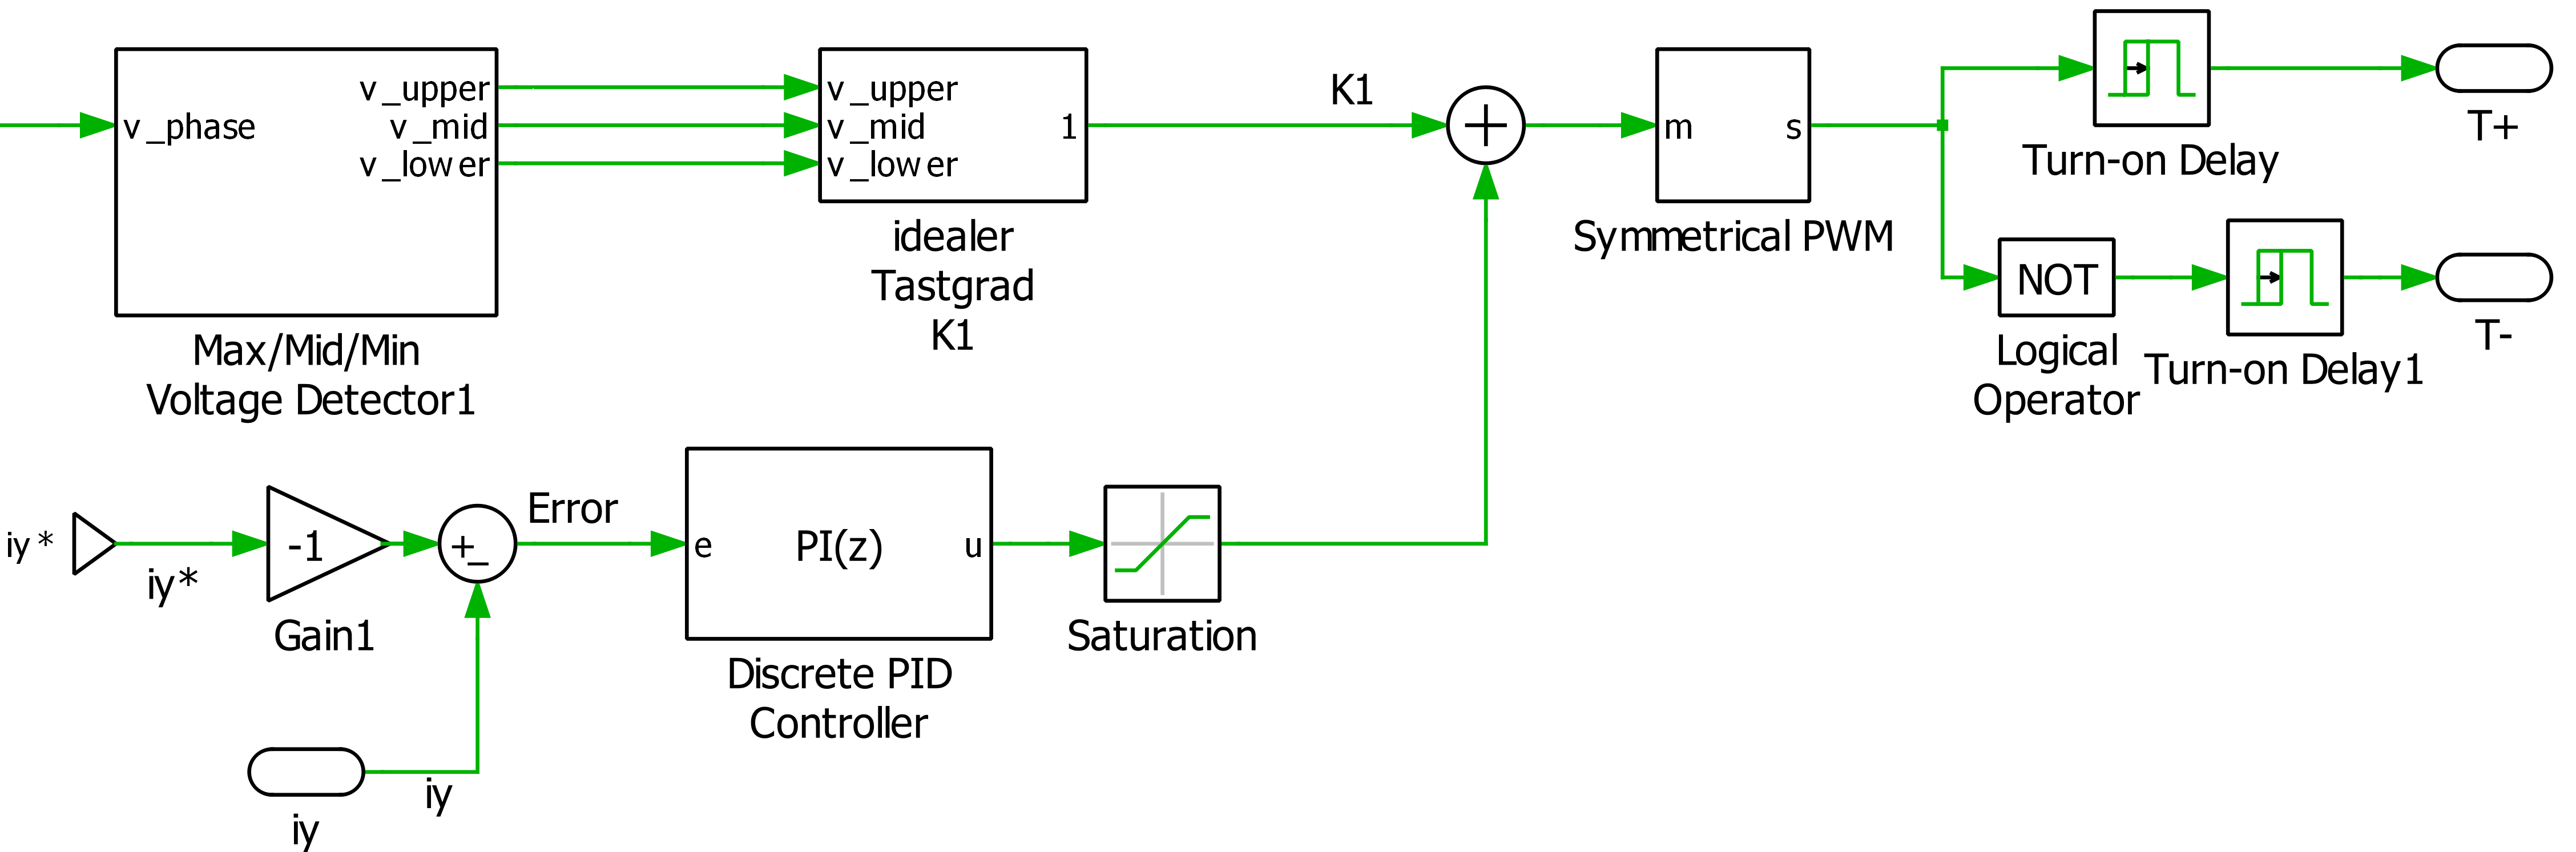
\includegraphics[width=1\linewidth]{content/Grafiken/PlecsIAFivsK1}
			\caption{Regelung des Stroms in der mittleren Phase}
			\label{fig:plecsiafivsk1}
		\end{figure}
		
	

\section{B6-1/3-PWM PFC Buck}
Die in Kapitel \ref{sec:GrundlagenB6} beschriebene Schaltung wird mit insgesamt drei Halbbrückenmodulen der Firma Infineon realisiert, siehe Abb. \ref{fig:plecsb6}. Es handelt sich dabei um weit verbreitete 1200 \si{\volt} Module, die einen nominellen Einschaltwiderstand von 2 \si{\milli \ohm} haben und Spitzenströme bis zu 800 \si{\ampere} schalten können \cite{IFAGFF2}.
\begin{figure}[H]
	\centering
	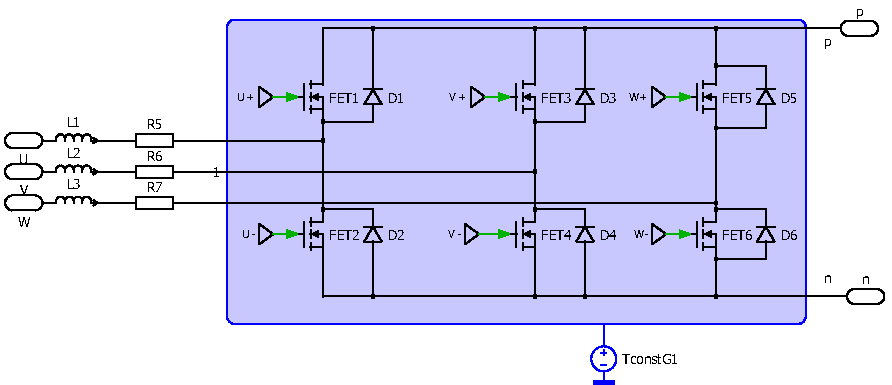
\includegraphics[width=1\linewidth]{content/Grafiken/PLECS_B6}
	\caption{PLECS Aufbau der B6 Leistungshalbleiter}
	\label{fig:plecsb6}
\end{figure}
 Um die Ausgangsleistung auch bei geringerer Spannung bereitzustellen zu können sind für den Tiefsetzsteller zwei Halbbrücken vorgesehen. Die Schaltung ist in Abbildung \ref{fig:plecsb6buck} zu finden. Es ist erkennbar, dass der Tiefsetzsteller durch die Kondensatoren am Eingang von der B6-Struktur entkoppelt ist.
 \begin{figure}[H]
 	\centering
 	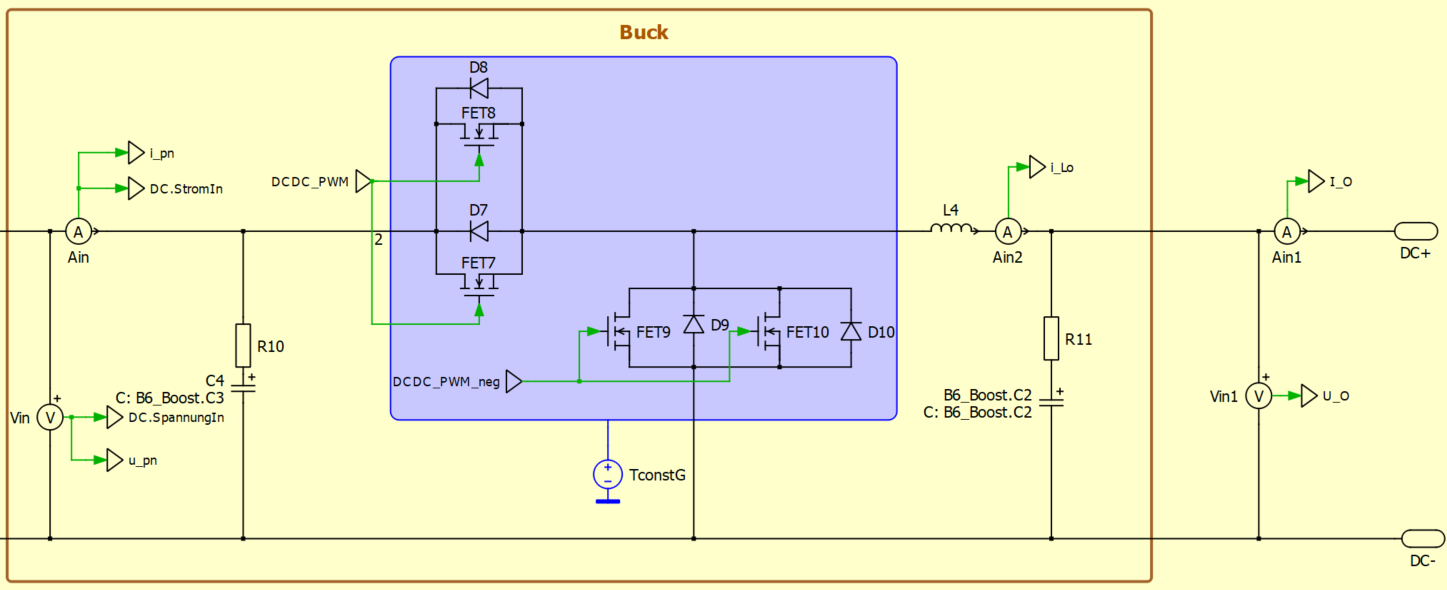
\includegraphics[width=0.9\linewidth]{content/Grafiken/PLECS_B6Buck}
 	\caption{PLECS Aufbau des Tiefsetzstellers der B6 Topologie}
 	\label{fig:plecsb6buck}
 \end{figure}
 

		\subsection{Auslegung der Netzinduktivität}
			Aufgrund der Begrenzung des Eingangsstroms muss die Drossel effizient ausgelegt werden, was zu einer Reduzierung der Ausgangsleistung bei Blindleistungsbereitstellung führt. Wie bereits in Abschnitt \ref{sec:AnfStromnetz} erläutert, ist dies vom Netzbetreiber gestattet. Der Rippelstrom in der Drossel wird wie zuvor auf 30 \% des Effektivstroms ausgelegt. Dieser erreicht bei einem Spannungseinbruch sein Maximum. Der Rippelstrom beträgt somit 88,2 Ampere, siehe Formel \ref{eq:DeltaI_B6}.\\
			
			\begin{equation}
				\label{eq:DeltaI_B6}
				I_{\Delta max B6}= \dfrac{0,3 \cdot \sqrt{2} \cdot P_{a}}{\sqrt{3}\cdot U_{LLmin}}= \dfrac{0,3\cdot \sqrt{2} \cdot 200 \si{\kilo \watt}}{\sqrt{3} \cdot 617 \si{V} \cdot 0,9} = 88,2 \si{\A}
			\end{equation}
			Die Induktivität kann nach der gleichen Beziehung wie für den \gls{IAF}-\gls{IVS} berechnet werden und beträgt 136 \si{\micro \henry}, siehe Formel \ref{eq:L_B6}.
			\begin{equation}
				\label{eq:L_B6}
				L_{B6}= \dfrac{U_{LLmaxPeak}}{4\cdot f{sw} \cdot I_{\Delta max B6}} = \dfrac{959,8V}{4 \cdot 20 kHz \cdot 88,2 A} =136 \si{\micro \henry}
			\end{equation}
			Die in der Induktivität gespeicherte Energie wird ebenfalls durch den Zusammenhang zwischen Netzspannung und Ausgangsleistung definiert, erhöht sich jedoch nicht durch die Bereitstellung von Blindleistung. Die gespeicherte Energie pro Phase beträgt 4,76 Joule nach Formel \ref{eq:EL_B6} und muss aufgrund der dreiphasigen Ausführung mit dem Faktor drei multipliziert werden. Somit ergibt sich eine Gesamtenergie von 14,28 Joule für die Hauptinduktivität der Topologie.
			
			\begin{equation}
			\label{eq:EL_B6}
			E_{LB6}= 3 \cdot 1/2 \cdot L_{B6} \cdot (\dfrac{\sqrt{2} \cdot P_{a}}{\sqrt{3}\cdot U_{LL}})^{2}= 3 \cdot 1/2 \cdot 136 \si{\micro \henry} \cdot ({\dfrac{\sqrt{2} \cdot 200 \si{\kilo \watt} }{\sqrt{3} \cdot 617 V}})^{2} = 14,28 J
			\end{equation}
			
			

		
		\subsection{Regelung}
			Die Regelung besteht aus einer vierstufigen Kaskadenstruktur, siehe Abbildung \ref{fig:b6-control-orig}. Die erste Stufe ist die Ausgangsspannungsregelung, die aus Sollleistung und Netzspannung die gewünschte äquivalente Phasenimpedanz als Eingangsgröße für die Phasenstromregelung bildet. Die drei Regler für die Phasenströme bilden die zweite Stufe\\
			In der dritten Stufe wird die Phase mit der mittleren Spannung ausgewählt und anhand der Phasenlage die Zwischenkreisspannung \gls{Upn} bestimmt. Die Zwischenkreisspannung ergibt sich als Sechspulsige-Gleichspannung und dient als Eingangsspannung für den Tiefsetzsteller. Die mittlere Phasenspannung wird als Referenz für den Tastgrad der entsprechenden Halbbrücke verwendet und prägt somit einen spannungsproportionalen Strom ein. Somit ist immer nur eine der drei Halbbrücken getaktet geschaltet, die anderen beiden sind wie bei einem Diodengleichrichter auf die jeweils positivste und negativste Spannung geschaltet.
			Die vierte Stufe ist der Tiefsetzsteller mit Reglern für den Eingangsstrom und die Ausgangsspannung.
				
			\begin{figure}[H]
			\centering
			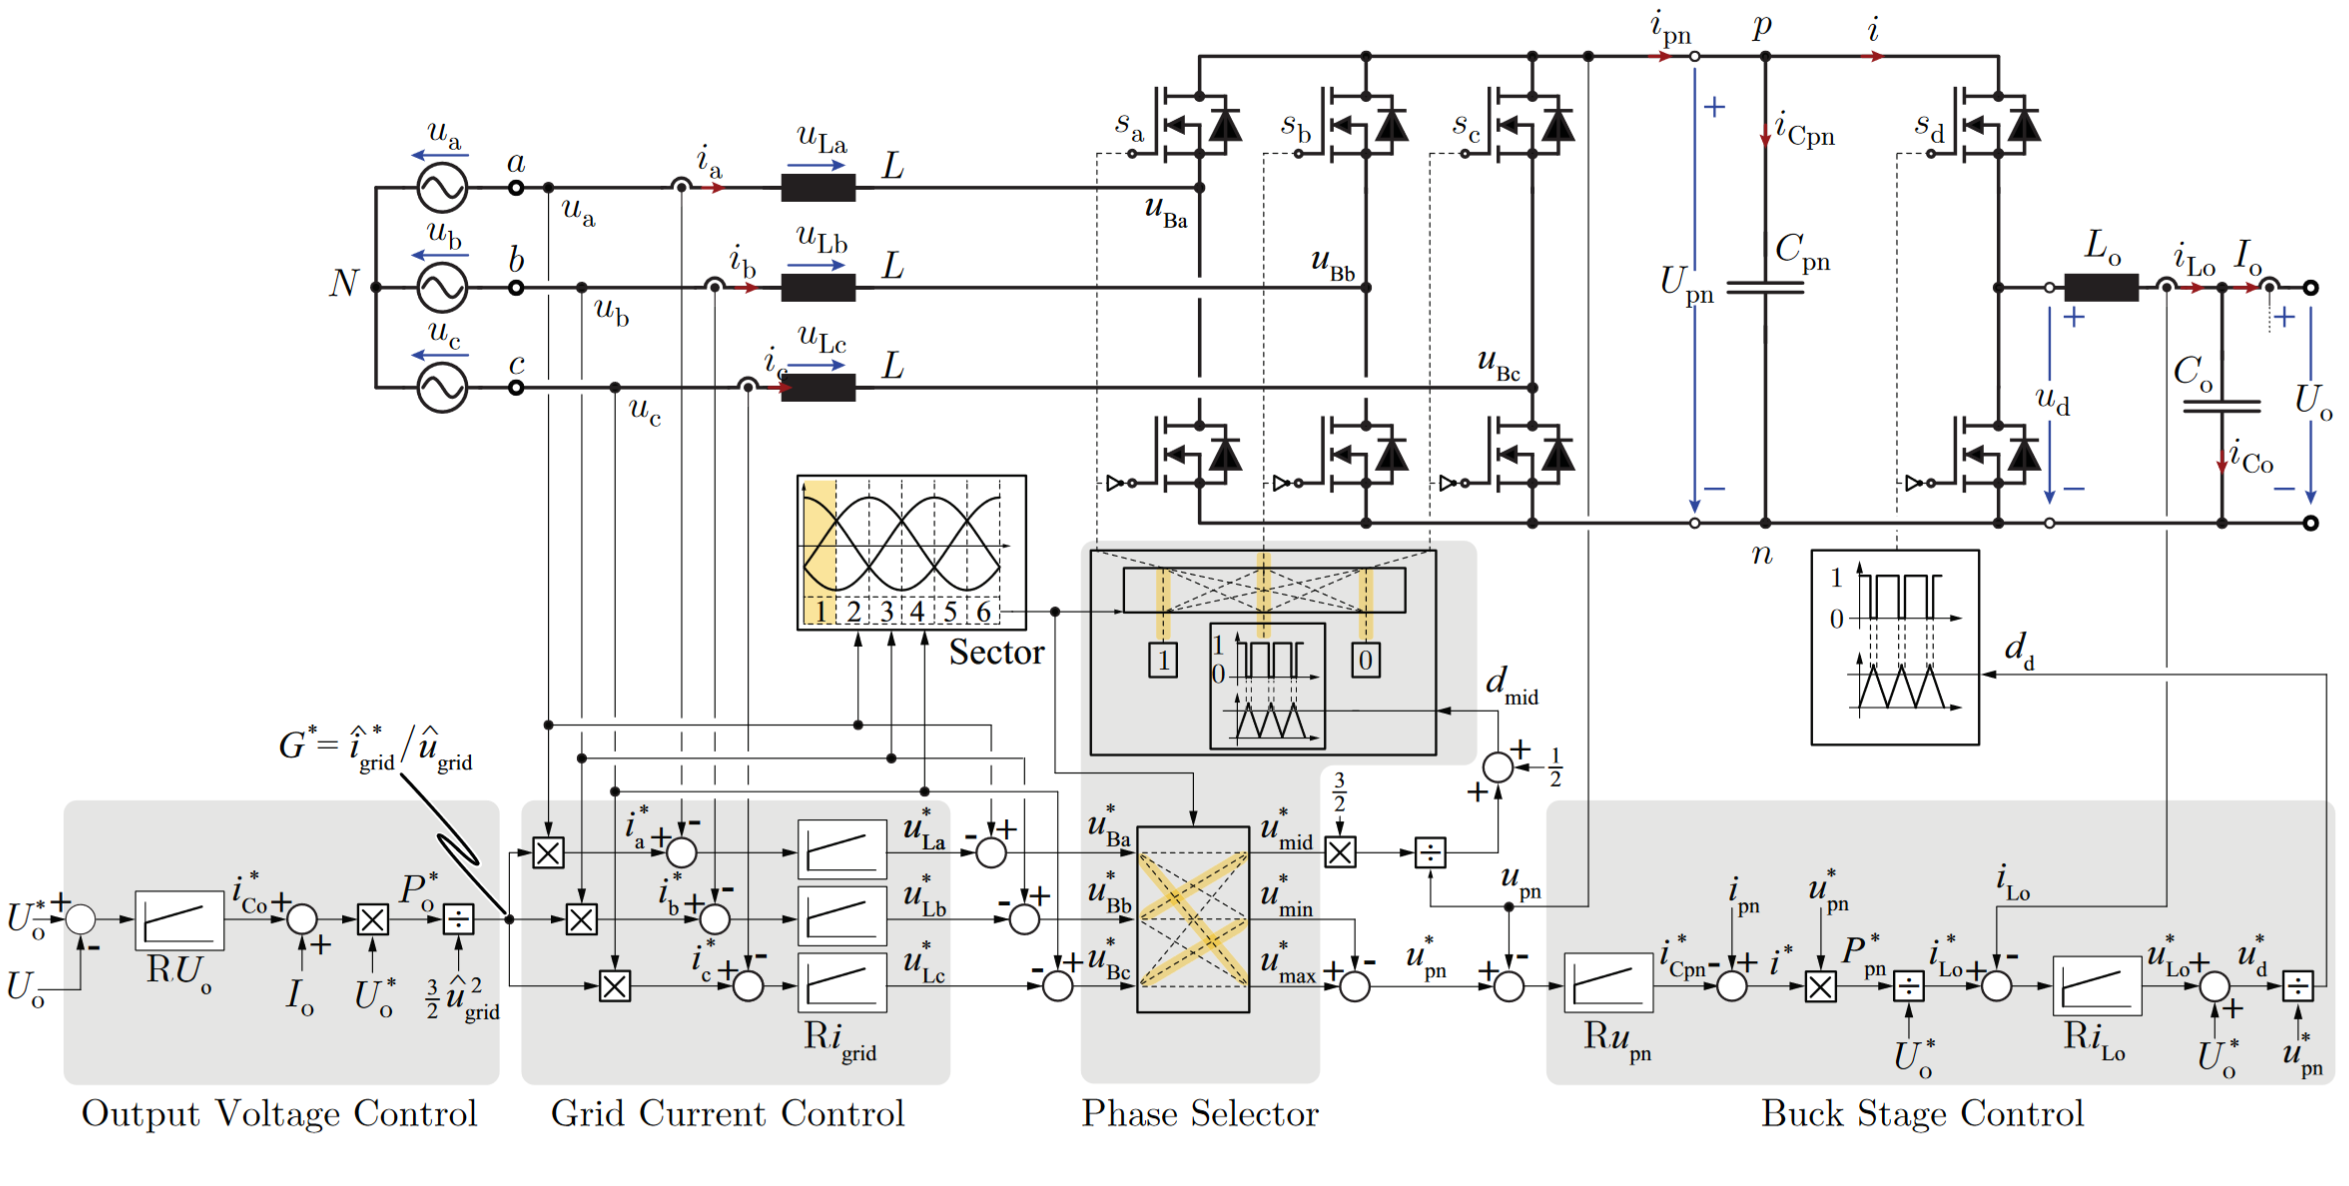
\includegraphics[width=0.9\linewidth]{content/Grafiken/B6-Control-orig}
			\caption{Regelung des \gls{B6PFC} \cite{13PWMPFC}}
			\label{fig:b6-control-orig}
			\end{figure}
		Die Ausgangsleistungsregelung in PLECS besteht aus einem PI-Regler (siehe Abbildung \ref{fig:plecsb6controlpout}), der die nominale Netzspannung mit der äquivalenten Netzimpedanz multipliziert und dann durch die aktuelle Netzspannung in die Soll-Phasenströme umgewandelt wird. Um die Phasenverschiebung zu implementieren, wird der Sollstrom entsprechend des Phasenwinkels verzögert an die Regelung der B6-Ansteuerung weitergegeben.\\
				\begin{figure}[H]
				\centering
				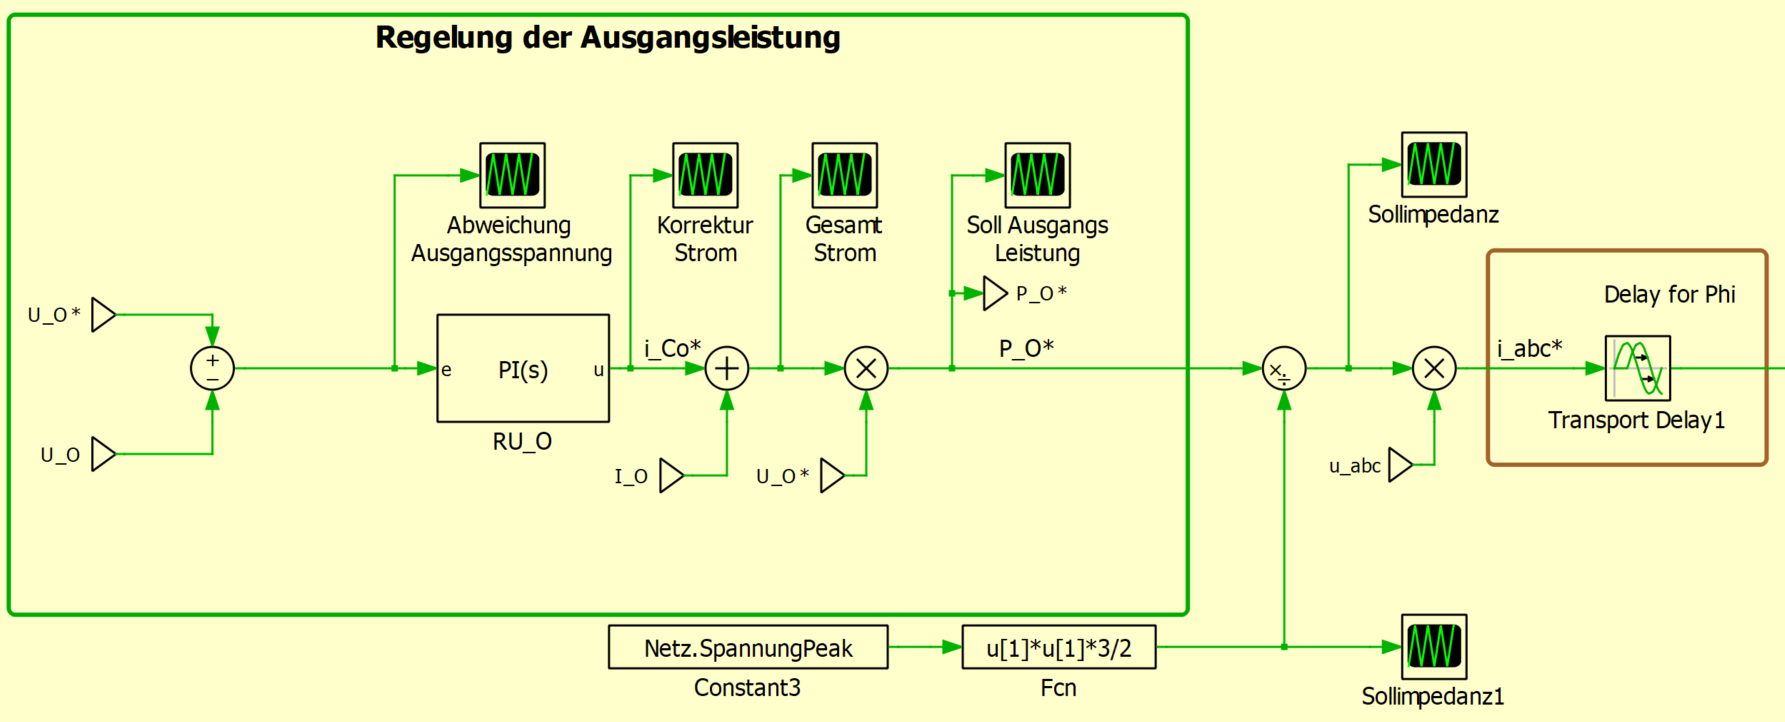
\includegraphics[width=0.9\linewidth]{content/Grafiken/PLECS_B6_ControlPout}
				\caption{PLECS Regelung der Ausgangsleistung als Sollgröße}
				\label{fig:plecsb6controlpout}
			\end{figure}
			Im nächsten Schritt wird die Regelung des Netzstroms durch einen weiteren PI-Regler implementiert. Die Erkennung der Phasenabschnitte wird mittels PLL und C-Skript umgesetzt. Siehe Abbildung \ref{fig:plecsb6controlrigrid}.  
				\begin{figure}[H]
				\centering
				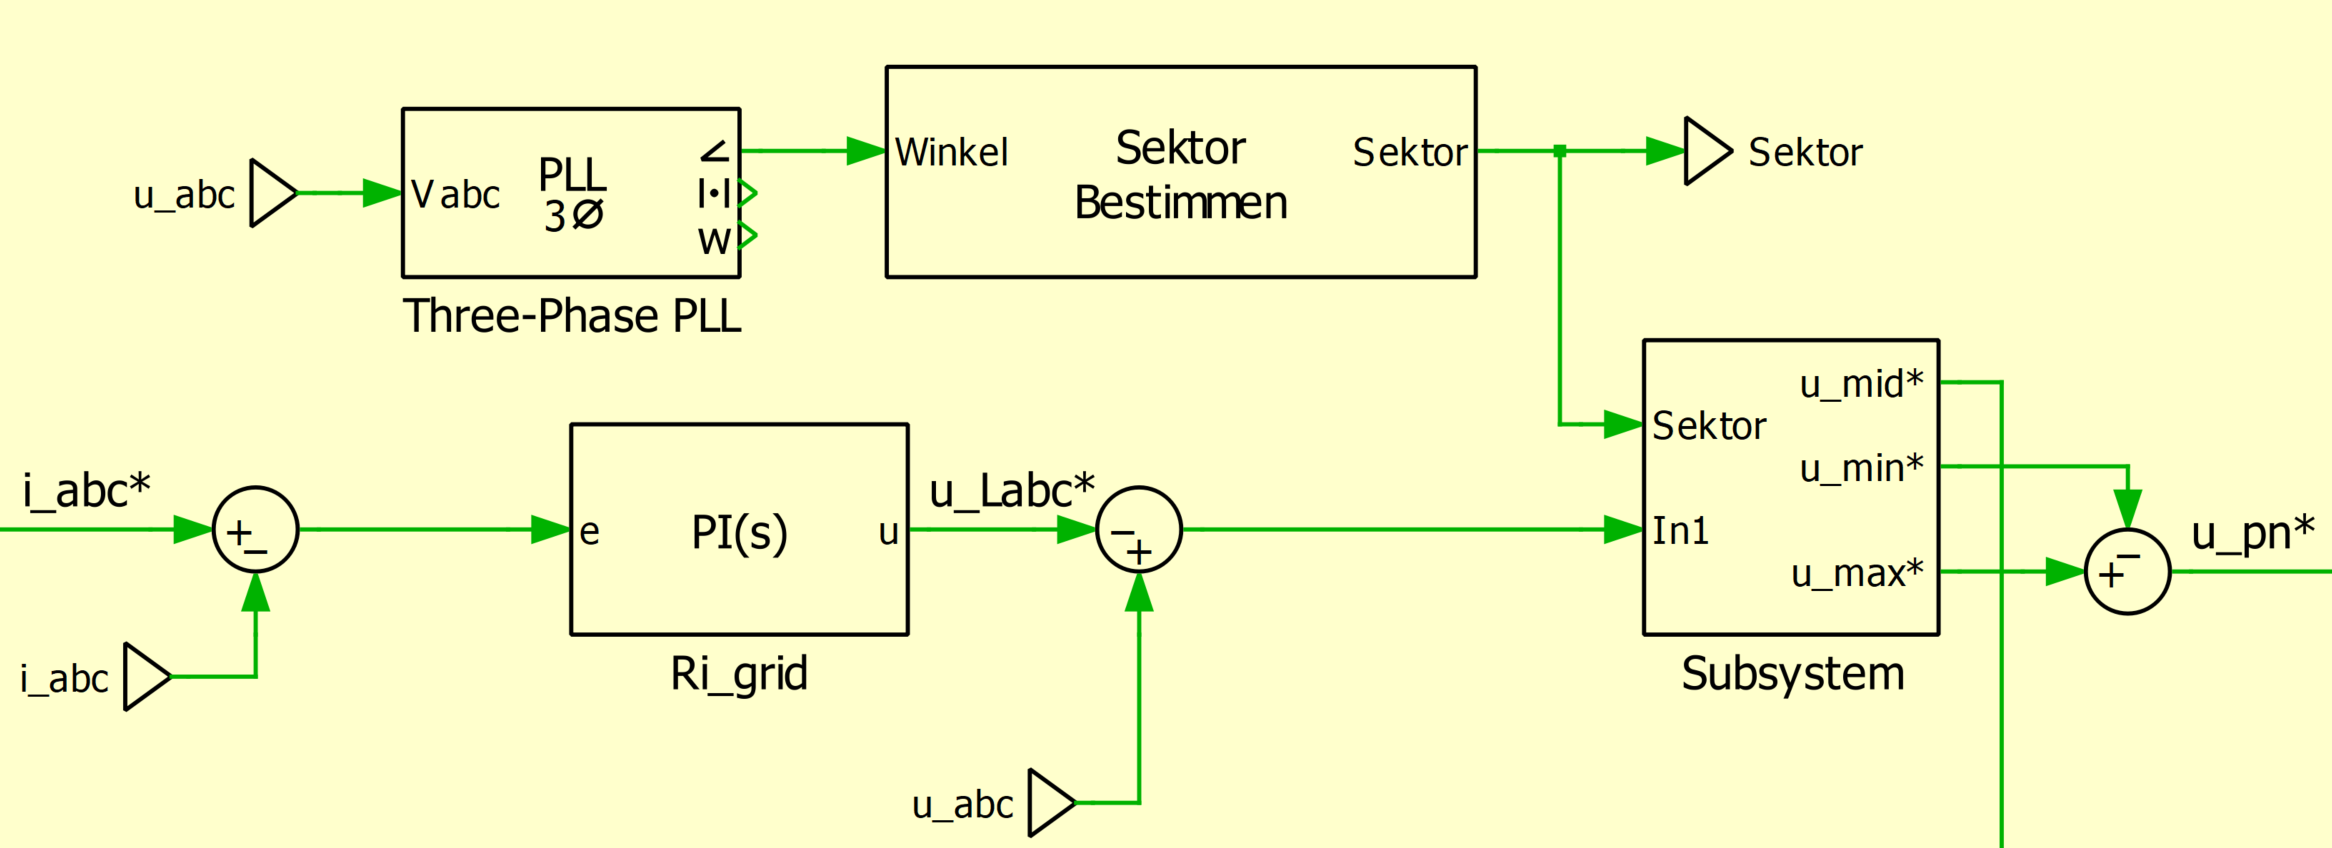
\includegraphics[width=0.9\linewidth]{content/Grafiken/PLECS_B6_ControlRiGrid}
				\caption{PLECS Regelung der Netzimpedanz und Phasenabschnittserkennung}
				\label{fig:plecsb6controlrigrid}
			\end{figure}
			Der Ausgang dieses Blocks dient einerseits mit \gls{Upn} als Eingang für den Tiefsetzsteller und andererseits wird die mittlere Spannung als Eingang für die PWM-Erzeugung des \gls{B6PFC} Gleichrichters verwendet. Die Ansteuerung des Tiefsetzstellers erfolgt wie in Abbildung \ref{fig:b6-control-orig} dargestellt, aus zwei PI-Reglern, die auf einen PWM-Generator geführt werden. Die Totzeit wird durch eine Einschaltverzögerung ergänzt.\\
			Zum anderen dient die Spannung der Mittenphase als Eingangsgröße zur Erzeugung des PWM-Signals für die \gls{MOSFET}s an der Mittenphase. Dieses wird wiederum von einem PWM-Generator erzeugt und mit Hilfe eines C-Codes werden die Signale den entsprechenden Phasen im Sektor zugeordnet. Die Einschaltverzögerung dient wiederum der Totzeit-Implementierung, siehe Bild \ref{fig:plecsb6controlpwmmid}.
			
		\begin{figure}
			\centering
			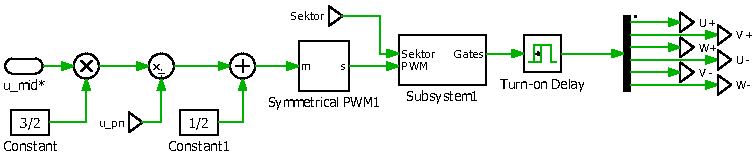
\includegraphics[width=0.9\linewidth]{content/Grafiken/PLECS_B6_ControlPWMmid}
			\caption{PLECS PWM Erzeugung des B6 Gleichrichters}
			\label{fig:plecsb6controlpwmmid}
		\end{figure}
		
		
			
			
